\subsection{Predictability of Group Archetypes}\label{apdx:replica_predictability}

\begin{figure}[h]
    \centering
    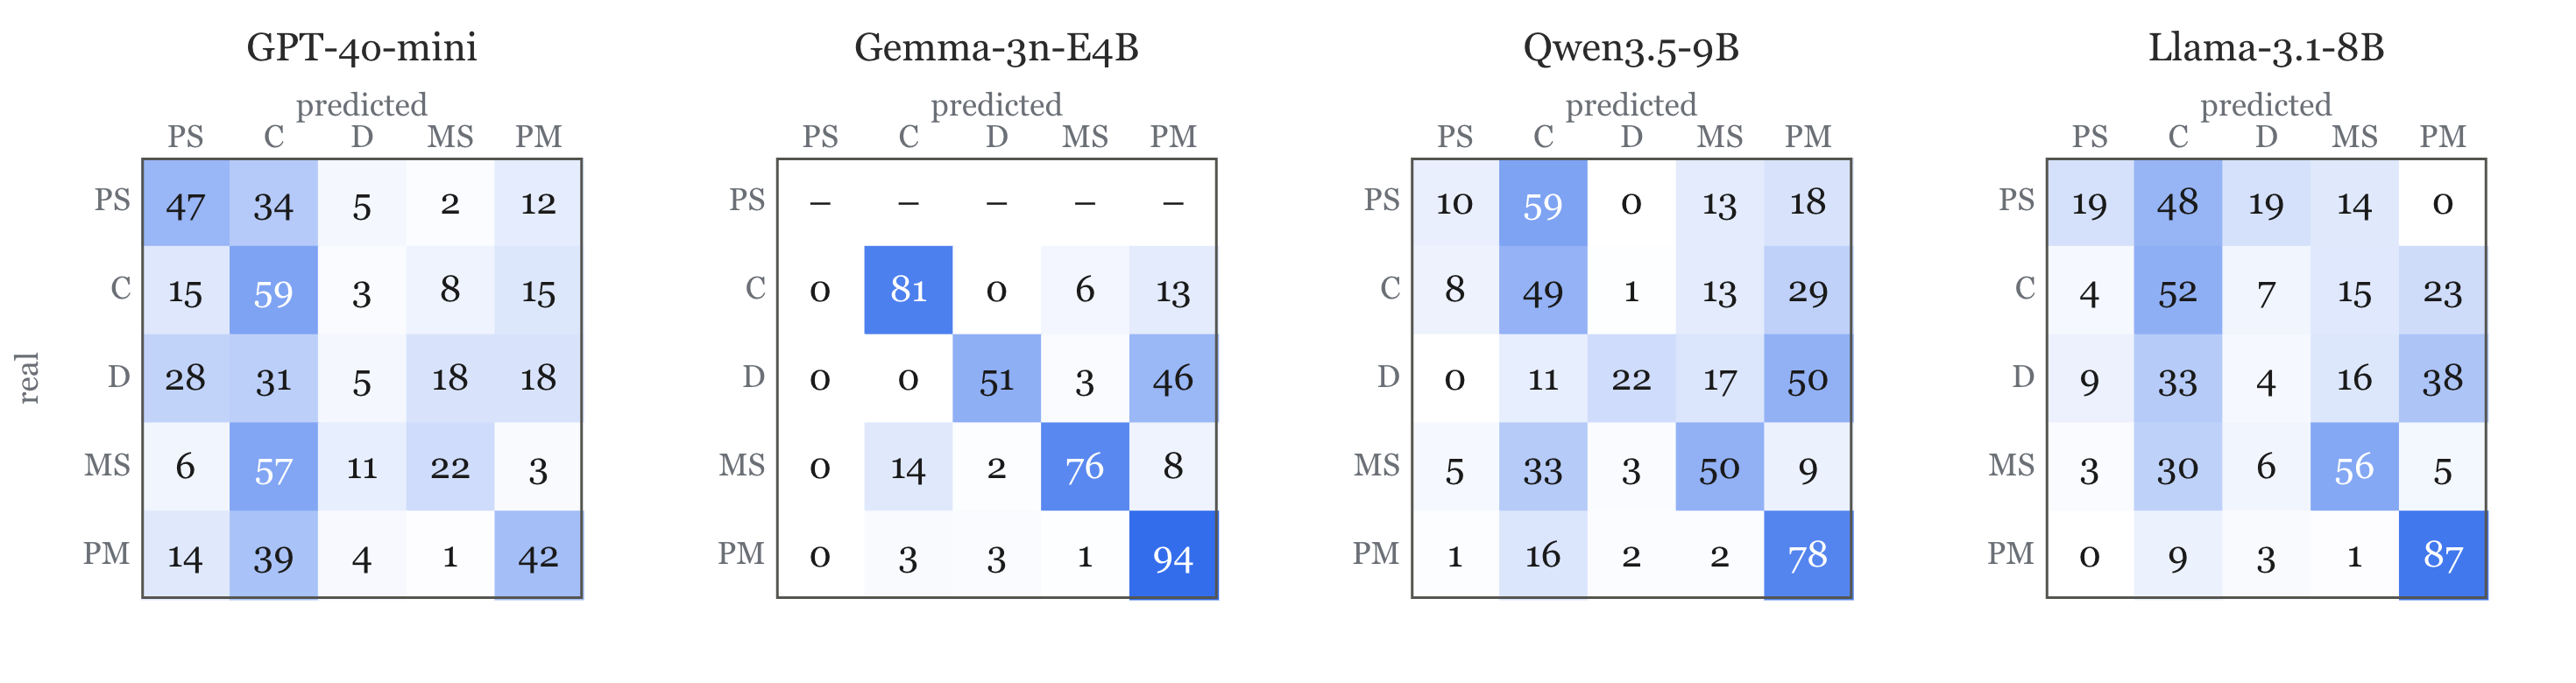
\includegraphics[width=0.99\textwidth]{main/Figures/apx_09_replica_predictability_objective.png}
    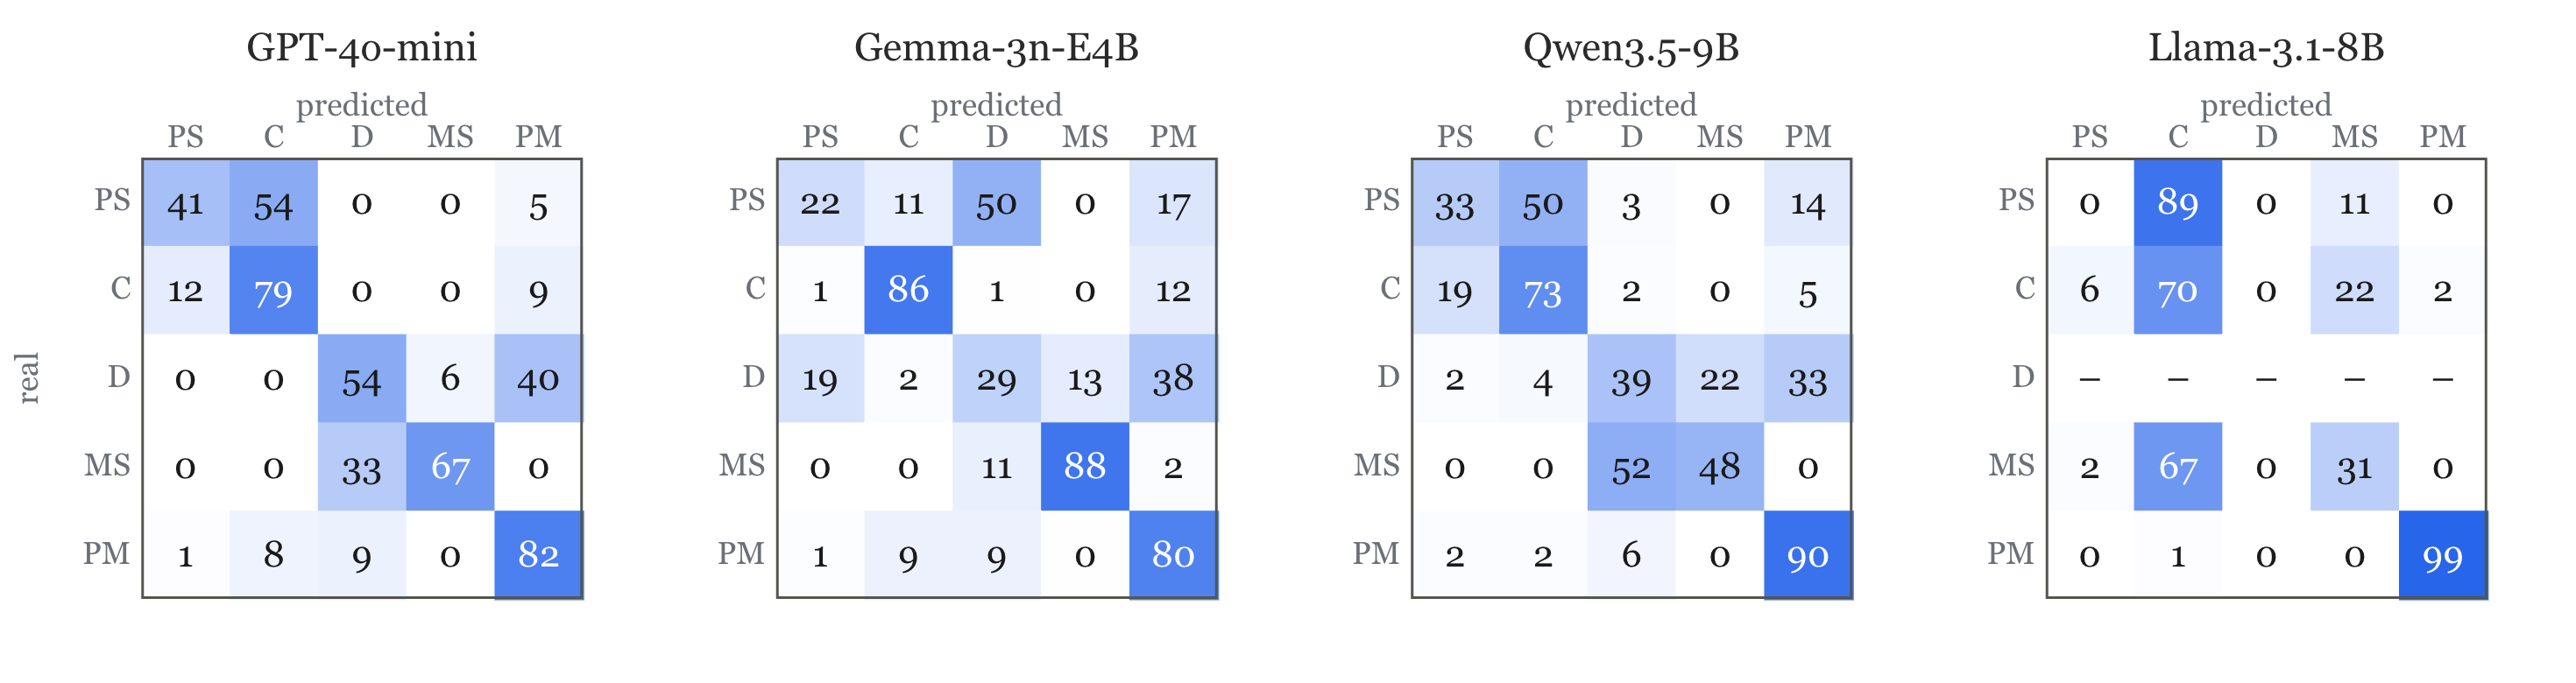
\includegraphics[width=0.99\textwidth]{main/Figures/apx_10_replica_predictability_subjective.png}
\caption{\textit{Predictability of the Group Archetypes (row 1: objective; row 2: subjective).} For every (question $\times$ graph) pair, we assess agreement among the $4$ independently sampled episodes. For this analysis, we use test questions and $4$ random graphs as our $J$s. For each question--$J$ pair, we use the group archetype of one of the $4$ trajectories as the predicted group archetype. We then use the remaining $3$ group trajectories as the test set to construct a confusion matrix for predicting the correct group archetype. We repeat this process, using each of the $4$ trajectories in turn as the prediction and the remaining $3$ as the test set, in a cross-validation manner, and report the \textit{``cross-validated''} confusion matrix. Because every trajectory takes its turn as the predictor, the cross-validated matrix is symmetric in raw counts. Row normalization makes the confusion matrix asymmetric. A row of the confusion matrix shows how often, for example, a \textit{persistent split} trajectory is predicted as each of the other group archetypes. If the repeated samples always matched, we would observe a diagonal confusion matrix with $100$ on the diagonal. \label{fig:predictability_macro_subjective_test_J03_cv_row}}\end{figure}
